\documentclass[aps,prl,twocolumn,superscriptaddress]{revtex4}
\usepackage{amsmath}
\usepackage{amsfonts}
\usepackage{amssymb}
\usepackage{bm}
\usepackage{dcolumn}
\usepackage{graphicx}
\usepackage[bookmarks,colorlinks]{hyperref}

\begin{document}
\title{Supplementary}

\date{\today}

\maketitle

In the commensurate charge-density-wave(CCDW) phase, $1T-TaS_2$ undergoes a commensurate reconstruction into a $\sqrt{13} \times \sqrt{13}$ super-lattice where 13 Ta atoms form a Star-of-David(SD) structure as illustrated in Fig. \ref{TBModel}. There are three inequivalent types of Ta atoms in the unit cell designated as "A", "B" and "C". The interatomic distances between "AB" and "BC" within the SDs shrunk by 6.4 and 3.2\%, respectively\cite{BROUWER198051}. In our study, we have ignored the slight non-radial movements of the atoms "B" and "C". After the reconstruction, the original nearest-neighbor bonds within the SDs are shorten and inter-cluster bonds are elongated. It is resonable to assign different hopping coefficients for bonds of different lengths. We also treat the center atoms specially, so the hopping coefficients on the "AB" bonds are independent from that on the "BB" bonds. To capture the essential physics, we propose the following Hubbard model for $1T-TaS_2$ in the CCDW phase:
\begin{equation}
H = -\sum_{<ij>\alpha} t_{ij} c_{i\alpha}^{\dagger} c_{j\alpha} + \sum_{i\alpha} \mu_i c_{i\alpha}^{\dagger} c_{i\alpha} + U\sum_{i} n_{i\uparrow} n_{i\downarrow} \label{model_Hamiltonian}
\end{equation}
where $<ij>$ indicates nearest-neighbors before the reconstruction, $t_{ij}$ the hopping amplitudes, $\mu_i$ the on-site energies and $U$ the on-site Coulomb interaction. The hopping coefficients for different bonds are explained in Fig. \ref{TBModel} and the chemical potential for atoms "A", "B" and "C" is $\mu_0$, $\mu_1$ and $\mu_2$ respectively.

The values of these tight-binding model parameters can be obtained by simulating the first-principle bands in the vicinity of $E_F$: $t_0=0.2, t_1=0.2, t_2=0.8, t_3=1.0, t_4=1.0, t_5=1.0, \mu_0=0.0, \mu_1=-0.6, \mu_2=-0.3$. The resulting bands and atomic-projected densities of states indicate that the states in the narrow split-off band are located preferentially on the central "A" atom of the Star-of-David cluster. As the band width is very small, the electron correlations many become dominant and the system is susceptible to a Mott-Hubbard transition.

To study the effects of electron correlation, we use cluster perturbation theory(CPT) \cite{PhysRevB.48.418,PhysRevLett.84.522} to process the Hubbard model. For our model, it is natural to choose the Star-of-David cluster as the CPT cluster and the effect of doping is reflected by putting different number of electrons into the cluster. Fig. \ref{ComposedDOS} shows the calculated density of states for different electron number at U=1.6. The tranfer of spectral weight from LHB to the bottom of UHB is compatible with the picture of electron doped Hubbard model. However, our experimental data shows that the additional excitation states appear at the top of LHB instead of the bottom of UHB. The incompatible between theoretical prediction and experimental observation implies that new physics may be reveled by our experiment.

\begin{figure}
    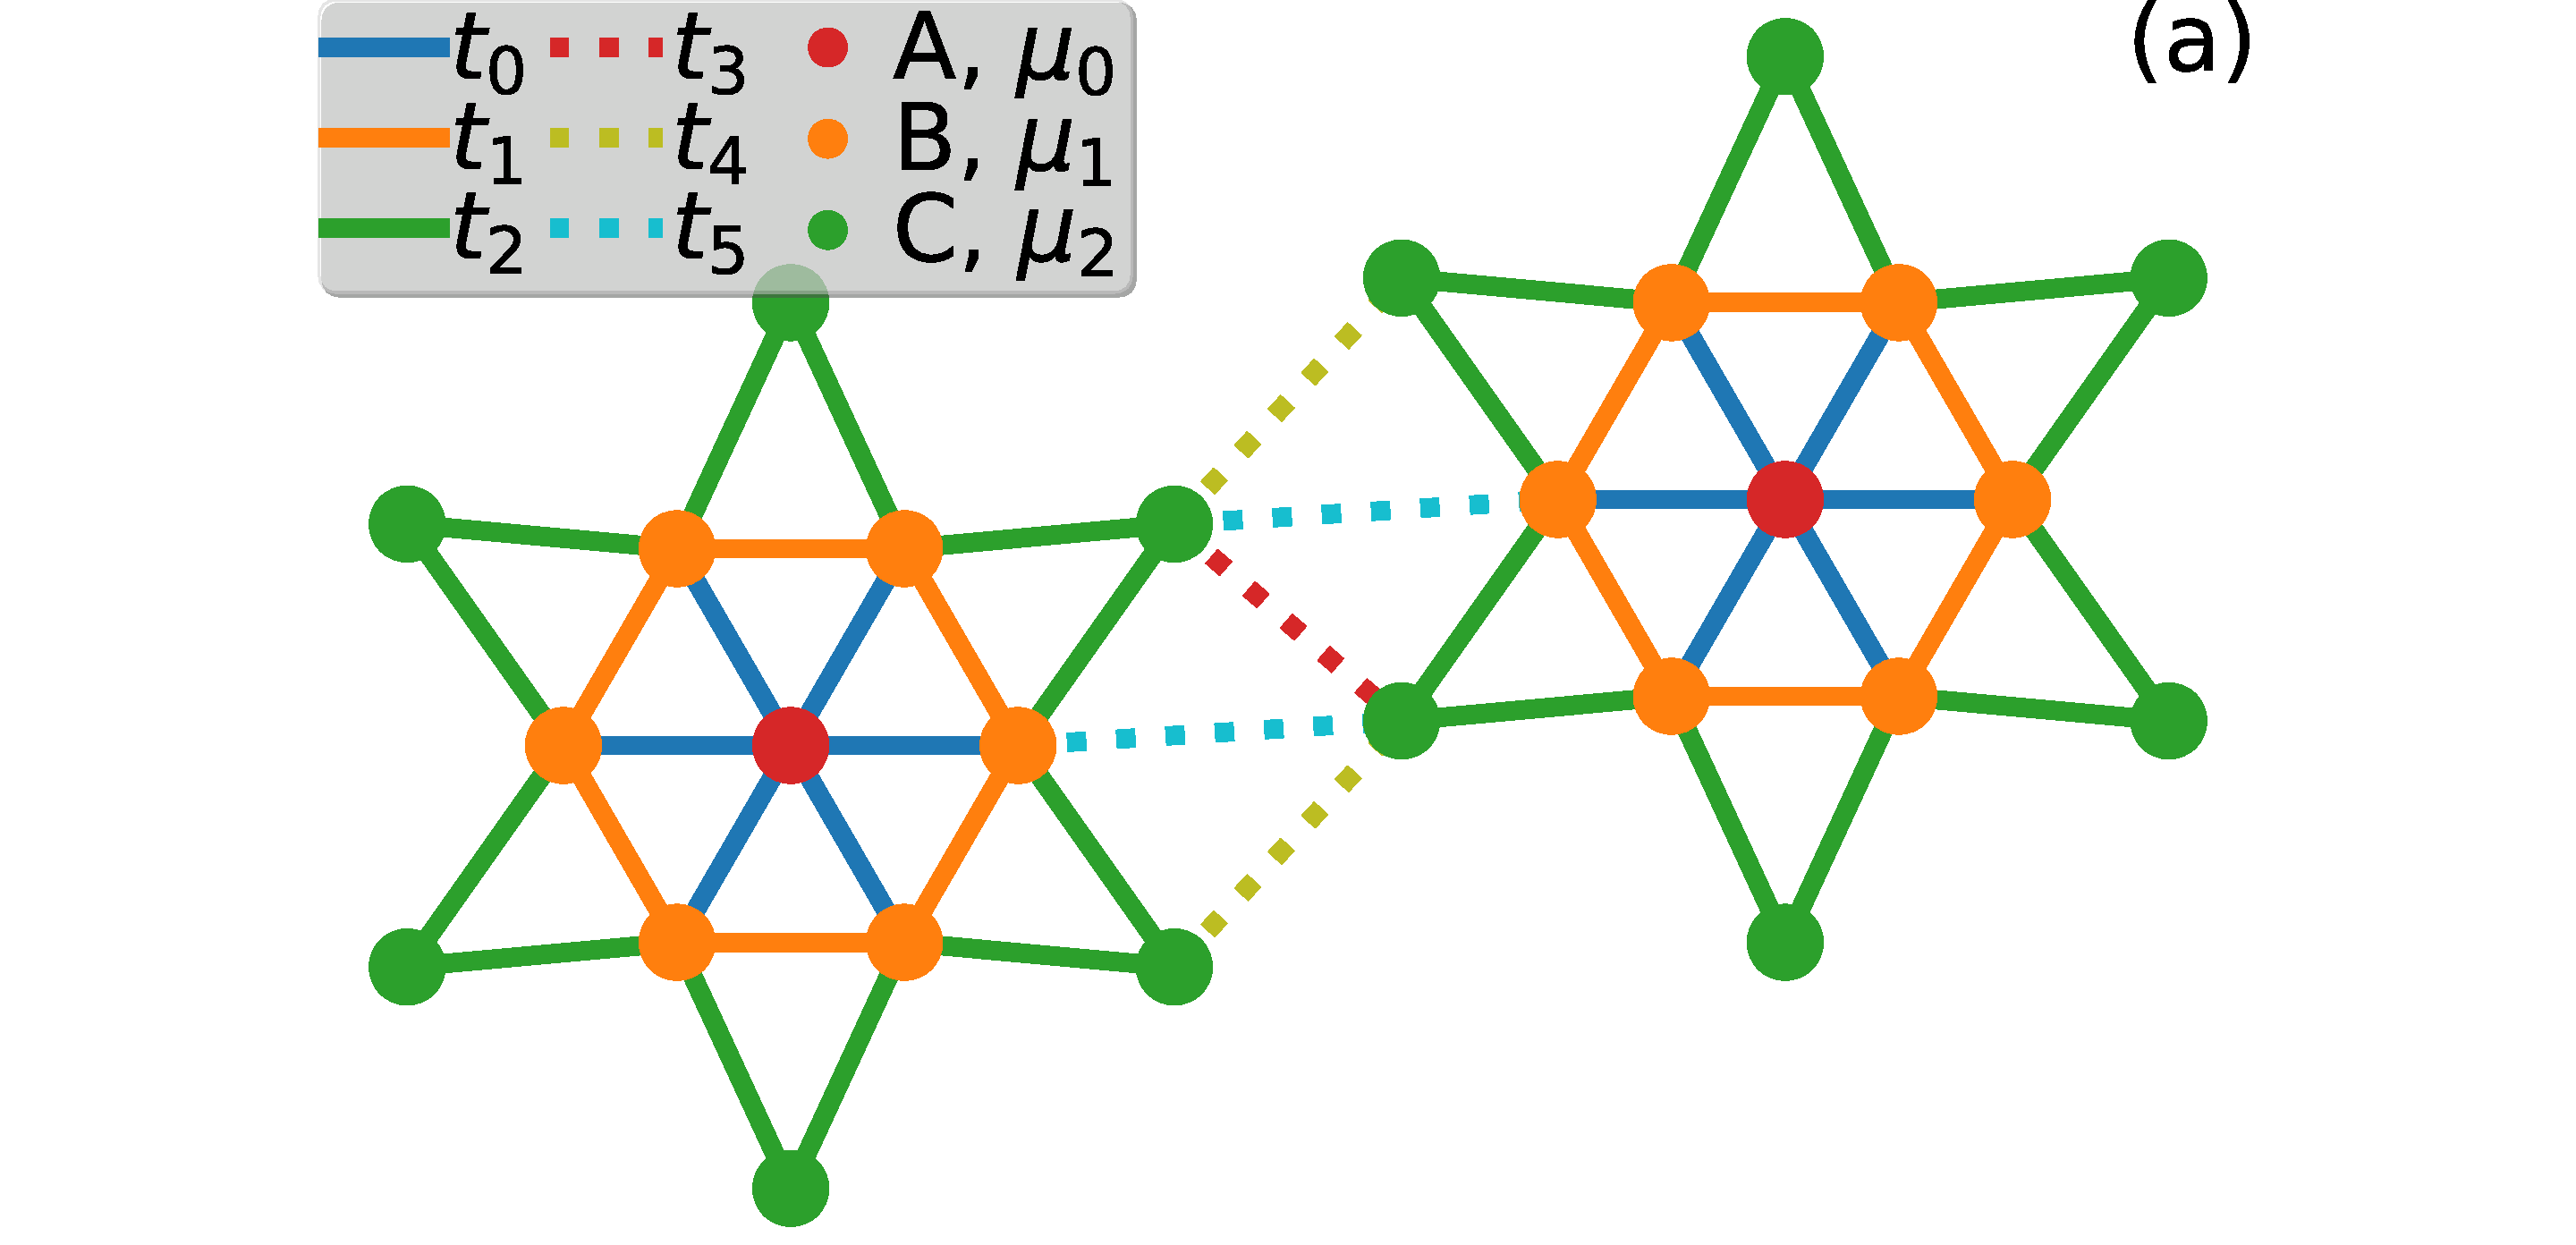
\includegraphics[width=\columnwidth]{StarOfDavidTB.pdf}
    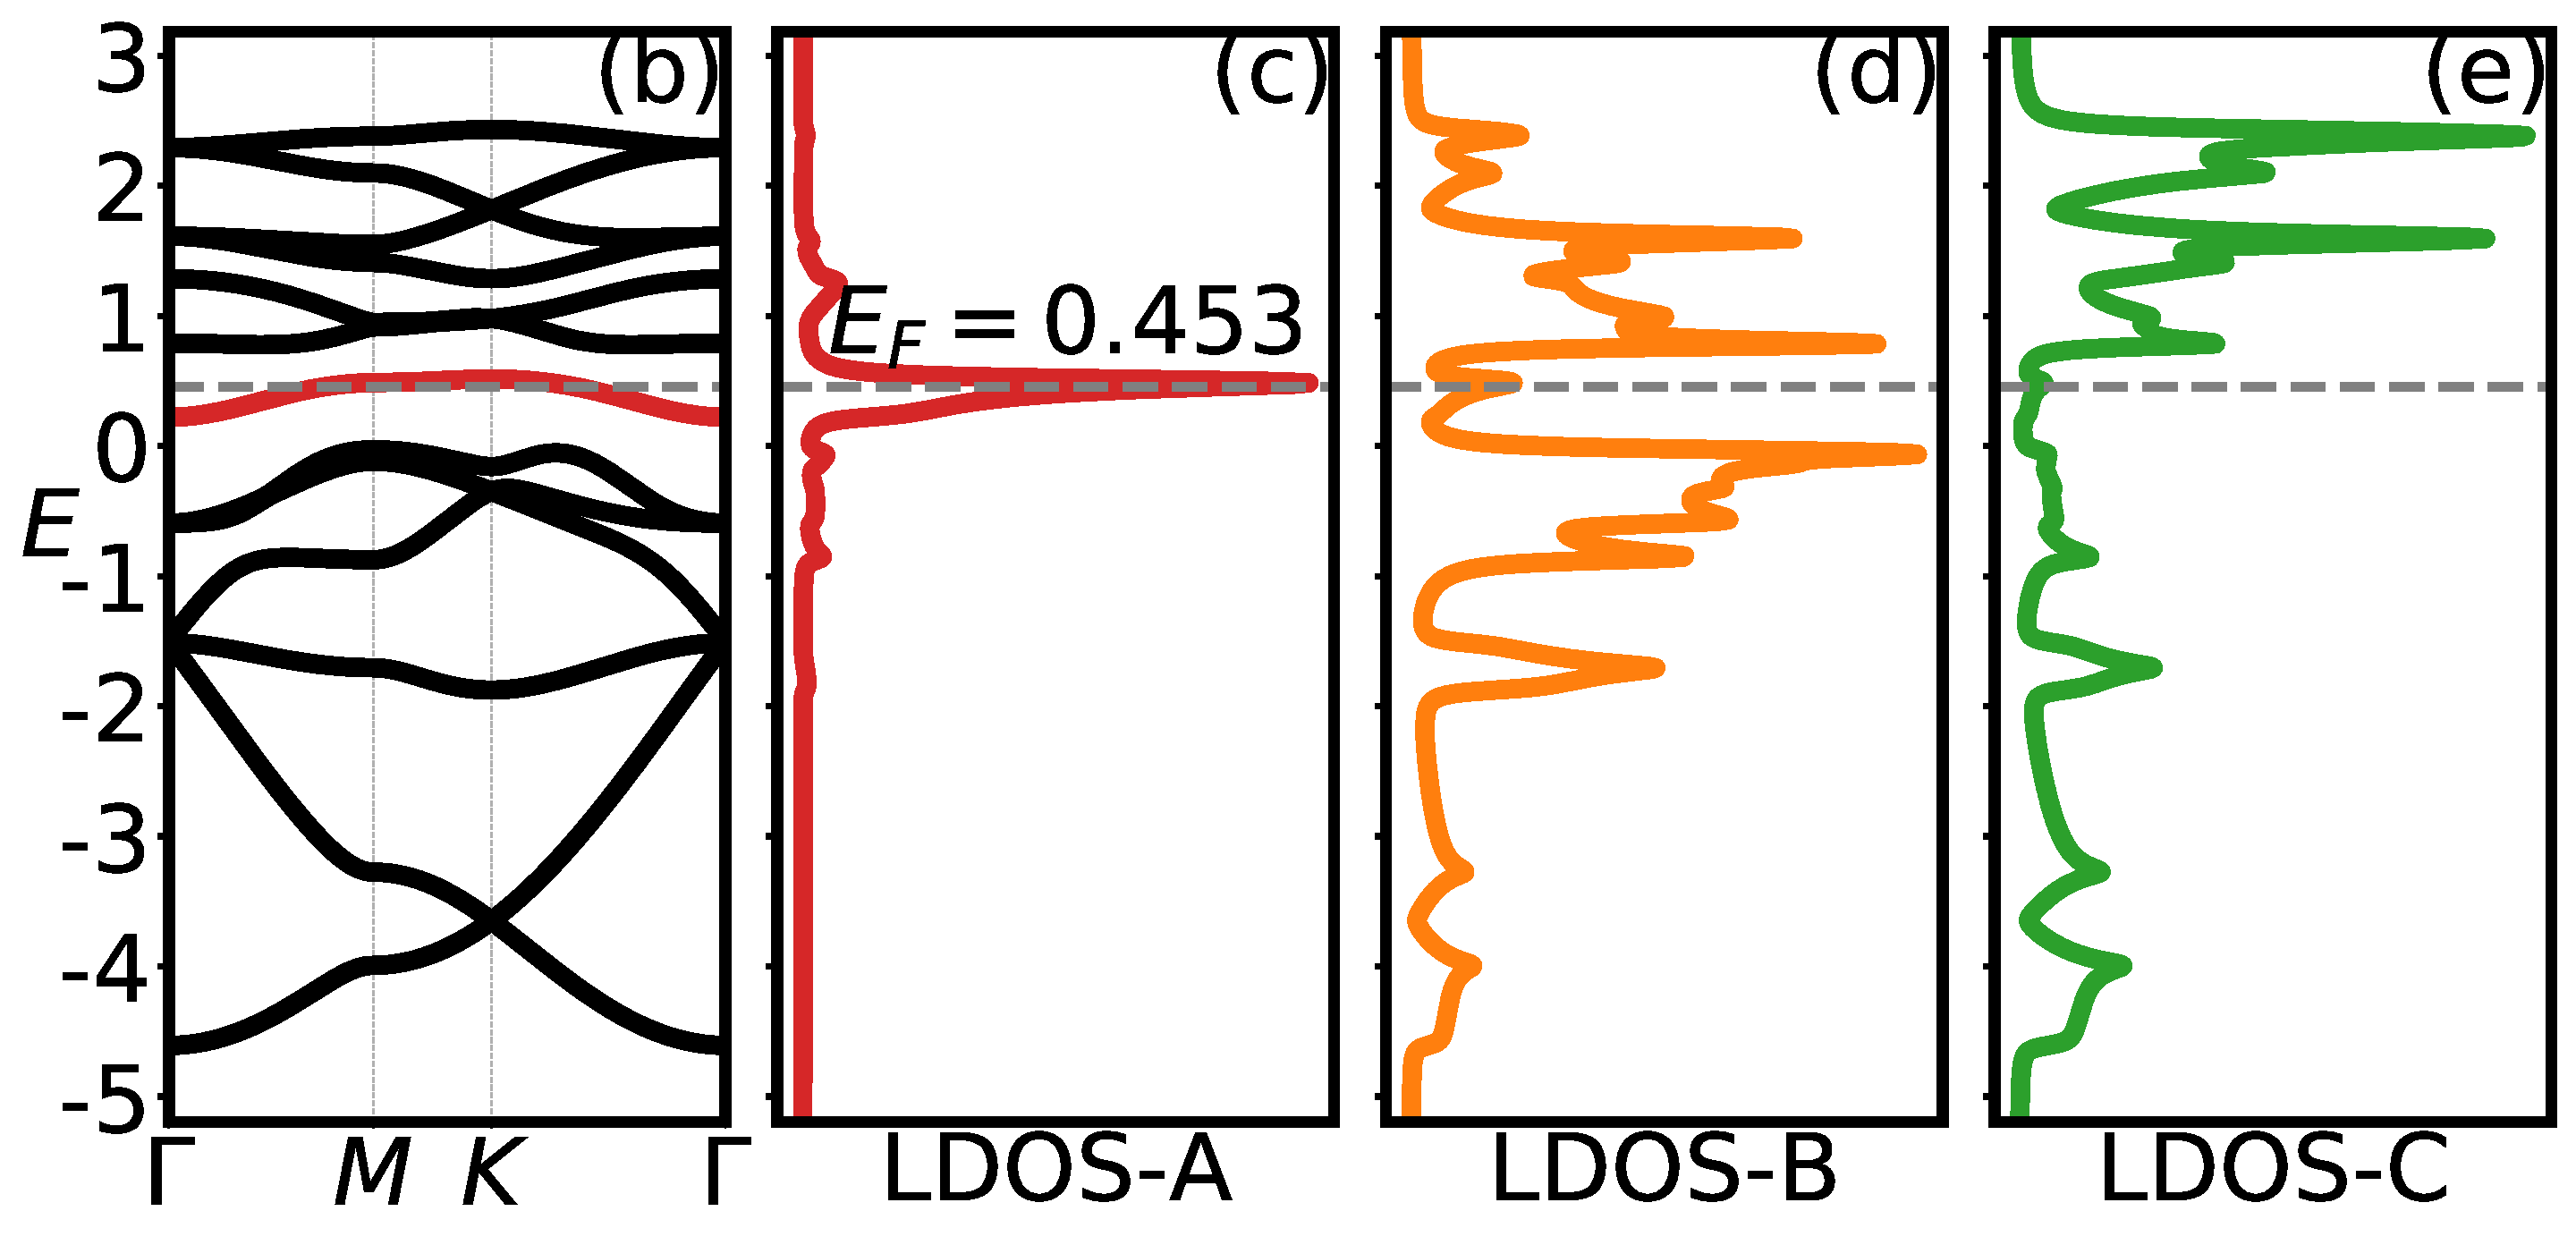
\includegraphics[width=\columnwidth]{EBAndDoS.pdf}
    \caption{\label{TBModel}Model definition and band structure. (a) SD unit cell and model parameter definition. These bonds with the same color have the same length and hopping coefficients. (b) The energy band at $t_0=0.2, t_1=0.2, t_2=0.8, t_3=1.0, t_4=1.0, t_5=1.0, \mu_0=0.0 ,\mu_1=-0.6, \mu_2=-0.3$. (c) - (e) The atomic projected densities of states for A-, B- and C-Type Ta atoms.}
\end{figure}

\begin{figure}
    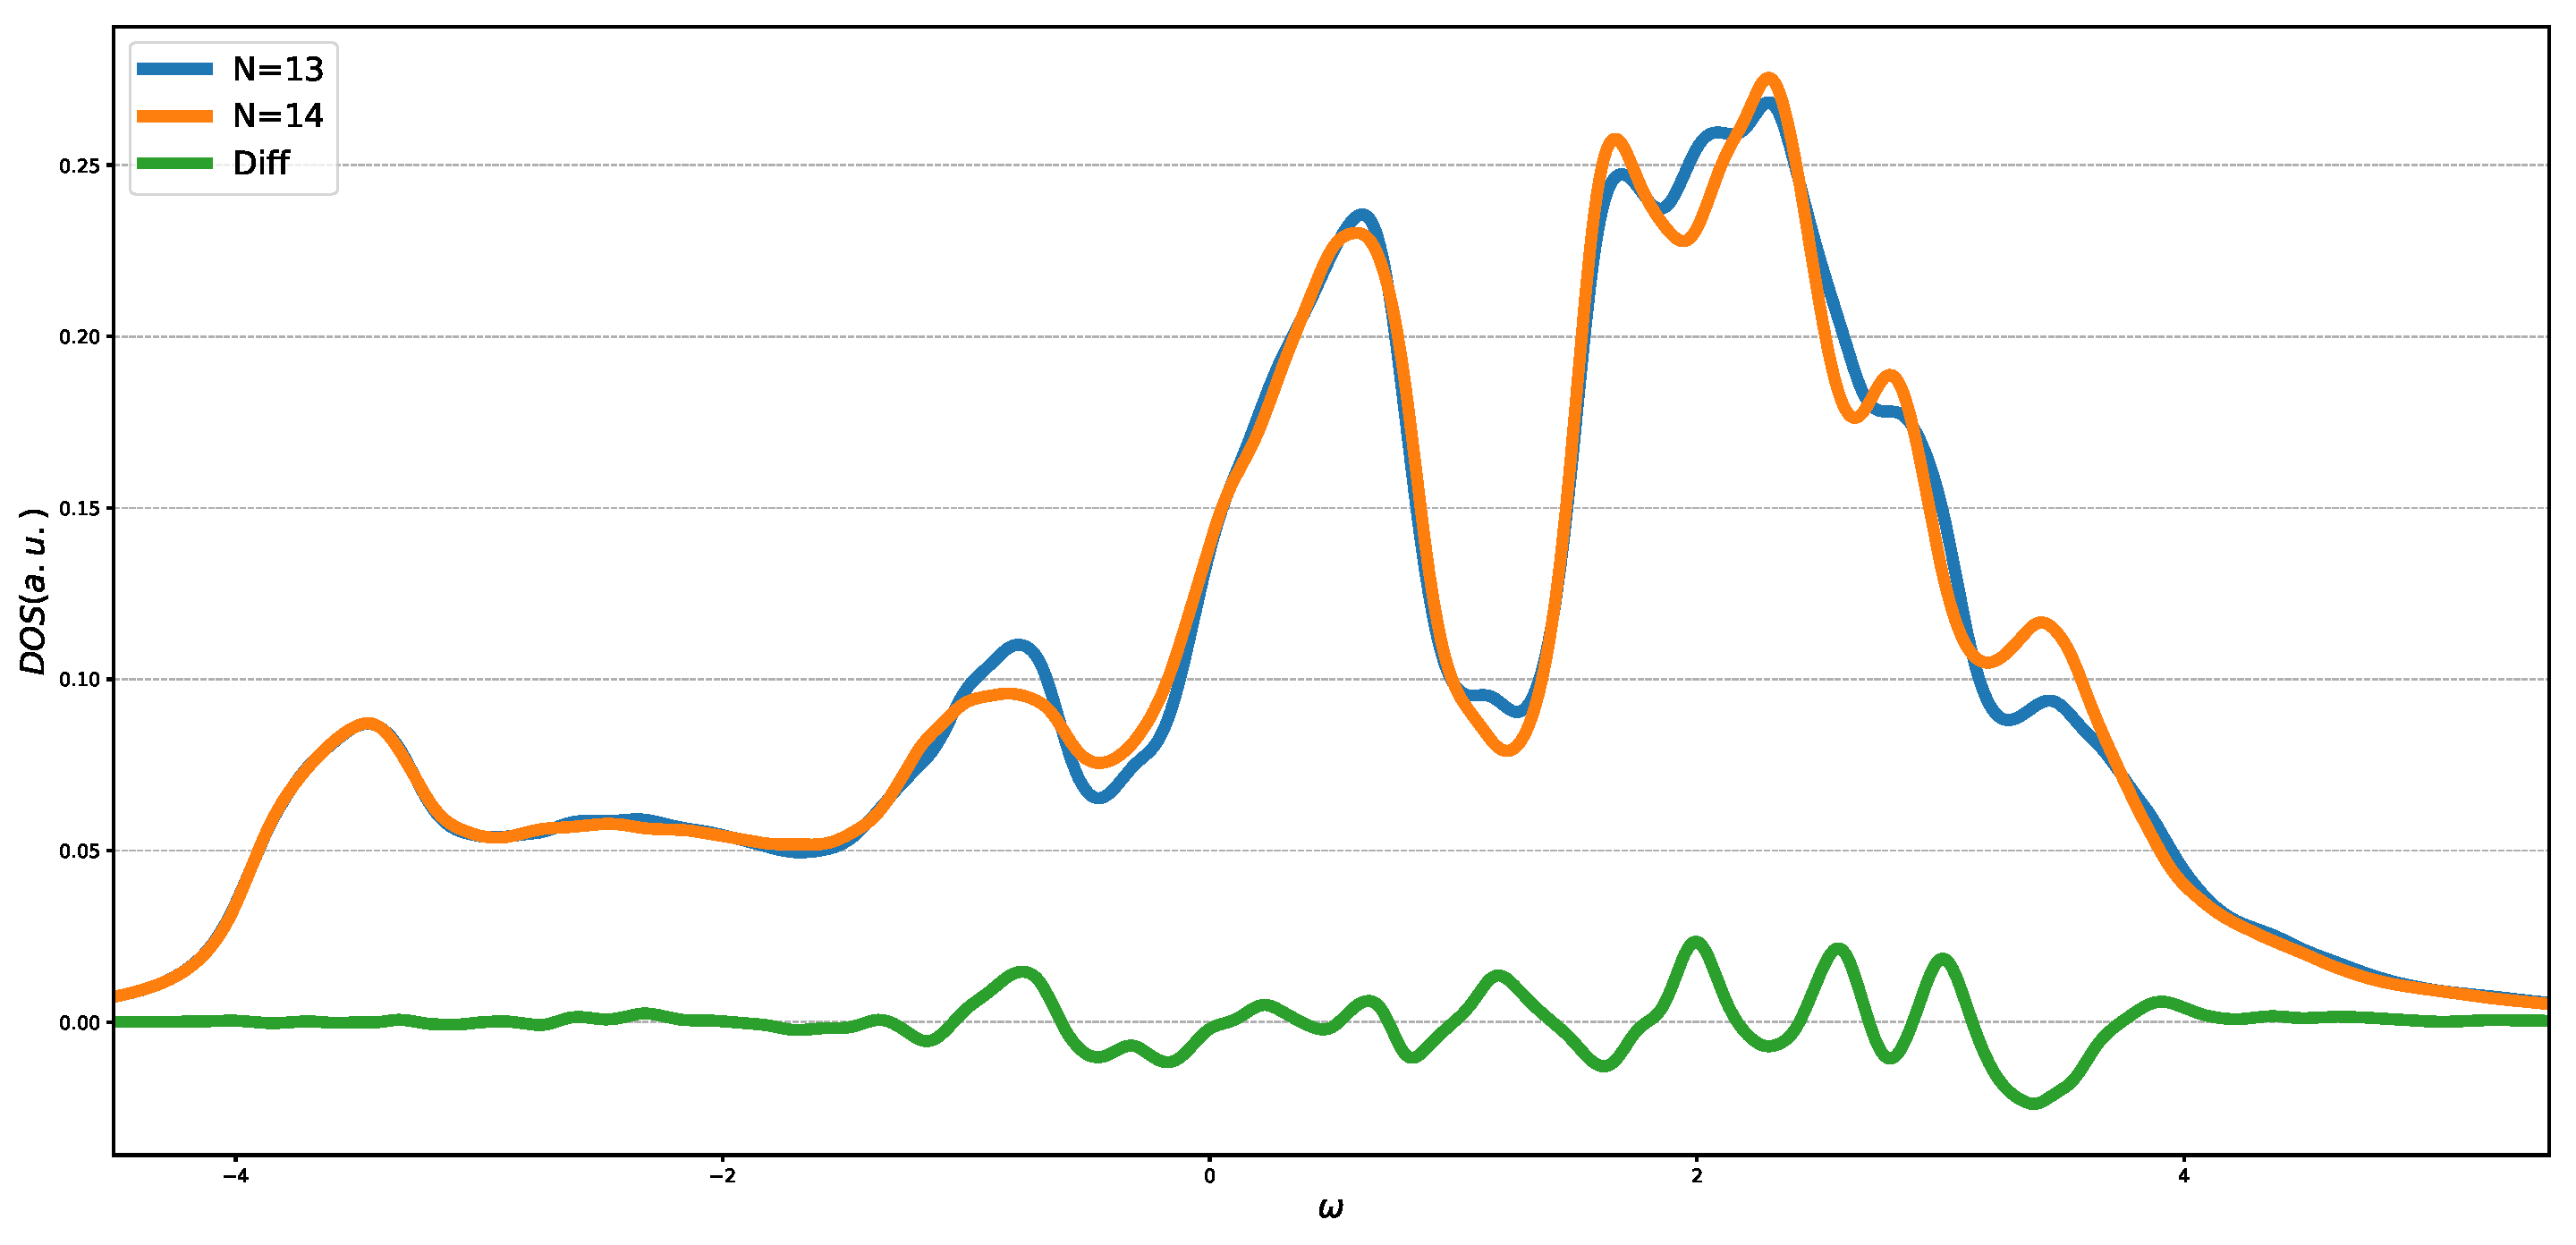
\includegraphics[width=\columnwidth]{ComposedDOS.pdf}
    \caption{\label{ComposedDOS}Density of states of the Hubbard model. The number of averaged electron per-unit-cell for the blue and orange line is 13 and 14, respectively. The green line shows the difference between the N=13 and N=14 case.}
\end{figure}

\bibliography{Supplementary}

\end{document}
